\documentclass[11pt,a4paper]{article}

% ----------------------------------------------------------------------
% Pacotes
% ----------------------------------------------------------------------
\usepackage[utf8]{inputenc}
\usepackage[T1]{fontenc}
\usepackage[brazil]{babel}
\usepackage[a4paper,margin=2.3cm]{geometry}
\usepackage{amsmath,amssymb}
\usepackage{booktabs}
\usepackage{graphicx}
\usepackage{subcaption}
\usepackage{algorithm}
\usepackage{algpseudocode}
\usepackage{microtype}
\usepackage{xcolor}
\usepackage[hidelinks]{hyperref}
\usepackage{caption}

\captionsetup{font=small,labelfont=bf}
\graphicspath{{figs/}}

% espaçamento confortável (limite de 13 páginas dá folga)
\setlength{\parskip}{3.5pt}
\renewcommand{\baselinestretch}{1.06}

\floatname{algorithm}{Algoritmo}
\renewcommand{\listalgorithmname}{Lista de Algoritmos}
\algrenewcommand\algorithmicrequire{\textbf{Entrada:}}
\algrenewcommand\algorithmicensure{\textbf{Saída:}}
\algrenewcommand\algorithmicwhile{\textbf{enquanto}}
\algrenewcommand\algorithmicdo{\textbf{faça}}
\algrenewcommand\algorithmicfor{\textbf{para}}
\algrenewcommand\algorithmicif{\textbf{se}}
\algrenewcommand\algorithmicthen{\textbf{então}}
\algrenewcommand\algorithmicelse{\textbf{senão}}
\algrenewcommand\algorithmicend{\textbf{fim}}
\algrenewcommand\algorithmicreturn{\textbf{retorne}}

% ----------------------------------------------------------------------
\title{\vspace{-1.2cm}\textbf{Análise de Risco Sistêmico na Cadeia de\\
Dependências do PyPI}}
\author{\normalsize\textbf{Matheus Farias Barbosa}\\[2pt]
\small MC859 --- Projeto em Teoria da Computação\\
\small \textit{UNICAMP}}
\date{1\textsuperscript{o} semestre de 2026}

\begin{document}
\maketitle
\vspace{-0.7cm}

\begin{abstract}
\noindent
Ataques à cadeia de suprimentos de software --- como a porta dos fundos plantada
no \texttt{xz-utils} em 2024 --- mostraram que comprometer um único pacote pouco
conhecido pode contaminar milhares de projetos que dependem dele indiretamente.
Este trabalho modela esse problema como um grafo de dependências do ecossistema
Python (PyPI) e constrói um \emph{pipeline} de quatro fases para identificar quais
pacotes representam os maiores pontos únicos de falha. A partir de dados reais do
BigQuery (\texttt{deps.dev} e contagens de download do PyPI), montou-se um grafo
com 4.427 pacotes e 47.568 dependências, calculou-se um score de risco e um índice
de criticidade para cada nó, simulou-se a propagação de uma vulnerabilidade pelo
Modelo de Cascata Independente e, por fim, confrontou-se o ranking resultante com
dados reais de CVEs do OSV.dev. O modelo se mostrou um excelente classificador de
priorização (\emph{Lift} de 6 a 11 vezes acima do acaso para vulnerabilidades de
alta severidade), embora não funcione como estimador contínuo de risco --- uma
limitação que, como se discute, decorre da própria natureza esparsa dos dados de
vulnerabilidade. O resultado mais marcante: comprometer o \texttt{typing-extensions}
contaminaria, em média, cerca de um terço de todo o grafo em pouco mais de três
saltos.
\end{abstract}

Repositório com código fonte: \href{https://github.com/Leibniz23/MC859---Projeto}{Link}

% ======================================================================
\section{Introdução e objetivos}
% ======================================================================

Praticamente nenhum software moderno é escrito do zero. Um projeto Python típico
declara meia dúzia de dependências diretas, mas cada uma delas traz consigo as suas
próprias dependências, e assim por diante, formando uma árvore que com frequência
ultrapassa a centena de pacotes de terceiros instalados sem que o desenvolvedor
sequer perceba. Essa comodidade tem um custo de segurança que ficou evidente em
episódios recentes: o caso \texttt{event-stream} no npm, o pacote \texttt{ctx}
sequestrado no PyPI e, sobretudo, a porta dos fundos inserida no \texttt{xz-utils}
em 2024, que por muito pouco não atingiu boa parte das distribuições Linux. Em todos
eles, o estrago potencial não vem da popularidade direta do pacote atacado, mas da
quantidade de projetos que dependem dele \emph{transitivamente}.

A pergunta que motiva este projeto é, portanto, estrutural: \textbf{dado o grafo de
dependências do PyPI, quais pacotes concentram o maior risco sistêmico?} Ou seja,
quais são os nós cuja contaminação se espalharia para a maior parte do ecossistema.
Trata-se de uma pergunta de priorização --- com recursos limitados de auditoria,
faz sentido olhar primeiro para os pacotes mais ``perigosos por posição''.

Os objetivos concretos do trabalho foram:

\begin{enumerate}\setlength\itemsep{1pt}
  \item Capturar dados reais de dependências e de uso (downloads) do PyPI e montar
        o grafo de dependências correspondente.
  \item Definir e calcular, para cada pacote, um \emph{score de risco} $R(v)$ e um
        \emph{índice de criticidade} $C(v)$ que combinem popularidade, centralidade
        e alcance na rede.
  \item Simular a propagação de uma vulnerabilidade a partir dos pacotes mais
        críticos, estimando o ``raio de impacto'' esperado de cada um.
  \item Validar o ranking produzido contra um \emph{ground truth} independente ---
        as vulnerabilidades reais (CVEs) registradas na base OSV.dev.
\end{enumerate}

O restante do relatório segue a ordem natural do \emph{pipeline}:
captura de dados (Seção~\ref{sec:dados}), construção e caracterização do grafo
(Seção~\ref{sec:instancia}), os algoritmos das quatro fases (Seção~\ref{sec:metodos}),
os resultados (Seção~\ref{sec:resultados}) e, finalmente, a análise crítica dos
achados (Seção~\ref{sec:analise}).

% ======================================================================
\section{Captura dos dados}\label{sec:dados}
% ======================================================================

Toda a etapa de coleta foi feita sobre conjuntos de dados públicos hospedados no
Google BigQuery, o que evitou a necessidade de \emph{scraping}. Foram duas fontes principais, mais uma terceira usada apenas na
validação.

\paragraph{Contagens de download (popularidade).}
A primeira consulta vai à tabela \texttt{bigquery-public-data.pypi.file\_downloads},
que registra cada download de um arquivo do PyPI. Agrupando por projeto numa janela
de 30 dias, obteve-se a contagem de downloads de cada pacote. Essa contagem cumpre
dois papéis: serve como critério de escolha dos pacotes-semente e, mais tarde, entra como o
componente de ``uso'' do score de risco. Os nomes são normalizados para
minúsculas, porque o PyPI trata \texttt{Requests} e \texttt{requests} como o mesmo
projeto e a base de dependências usa a forma canônica.

Vale registrar uma mudança em relação ao planejamento inicial, que previa coletar a
frequência de uso pela API do \texttt{pypistats.org}. Optou-se por substituí-la pelo
BigQuery por dois motivos. Primeiro, a API do pypistats impõe forte latência e limites
de requisição: baixar o histórico de milhares de pacotes, um a um, levaria tempo
demais e tornaria a coleta pouco eficiente. Segundo, no começo do projeto não se
sabia que o próprio BigQuery já expunha as contagens de download do PyPI na tabela
\texttt{pypi.file\_downloads}; ao descobrir isso no decorrer do trabalho, ficou claro
que concentrar as duas fontes --- uso e dependências --- numa única plataforma
simplificava o \emph{pipeline} e permitia obter tudo com uma só consulta, sem
\emph{scraping} nem espera por uma API externa lenta.

\paragraph{Arestas de dependência.}
A segunda fonte é o conjunto \texttt{deps.dev} da Google
(\texttt{bigquery-public-data.deps\_dev\_v1}), que mantém o grafo de dependências de
vários ecossistemas. Consultou-se a versão de \emph{release} mais recente de cada
pacote (usando \texttt{VersionInfo.Ordinal} para desempatar e descartando
pré-lançamentos) e extraíram-se todas as arestas \texttt{PYPI $\to$ PYPI}. O resultado
bruto foi bem maior do que o esperado: quase \textbf{9,8 milhões} de arestas de
dependência cobrindo todo o PyPI. Trabalhar com o grafo inteiro seria caro e, na
prática, pouco informativo --- a imensa cauda de pacotes obscuros adicionaria ruído
sem alterar a cabeça da distribuição, que é o que interessa.

\paragraph{Seleção das sementes e fechamento transitivo.}
Para recortar uma instância tratável, selecionaram-se os \textbf{5.000} pacotes mais
baixados como sementes e, a partir deles, fez-se uma busca em largura (BFS)
seguindo as arestas de dependência até as folhas. Em outras palavras: parte-se dos
pacotes que as pessoas realmente usam e desce-se por toda a sua árvore de
dependências, recolhendo todo nó alcançável e toda aresta entre nós visitados.
Esse fechamento transitivo é o que define a instância de trabalho. A intuição é que
um pacote só importa para a análise se algum pacote popular depender dele,
direta ou indiretamente.

\paragraph{Ground truth de vulnerabilidades.}
Por fim, para a validação (Fase 4), consultou-se a API REST do
\textbf{OSV.dev}, um agregador aberto de \emph{advisories} de segurança mantido pela
Google. Como são milhares de pacotes a consultar, usou-se a rota \texttt{querybatch}
para descobrir baratamente quais pacotes têm \emph{algum} aviso e só então se buscam
os detalhes completos desses, evitando milhares de requisições vazias. De cada
\emph{advisory} extrai-se o score CVSS por uma estratégia de três níveis (parsing
do vetor CVSS v3/v4/v2; se ausente, mapeamento do rótulo textual de severidade; se
nada disso existir, descarta-se o score mas ainda se conta a vulnerabilidade).

% ======================================================================
\section{Construção e caracterização da instância}\label{sec:instancia}
% ======================================================================

O grafo é dirigido: uma aresta $u \to v$ significa ``\,$u$ depende de $v$\,''. Cada
nó recebe como atributo a sua contagem de downloads, que passa por uma transformação
$\log_{10}(1+x)$ seguida de normalização min--max para o intervalo $[0,1]$. O
logaritmo é essencial aqui porque a distribuição de downloads é extremamente
desigual --- os pacotes do topo recebem ordens de grandeza mais tráfego do que a
mediana, e sem a compressão logarítmica o score de uso ficaria dominado por meia
dúzia de gigantes.

A instância final tem \textbf{4.427 nós e 47.568 arestas} (densidade
$\approx 0{,}0024$). Três propriedades estruturais dela condicionam tudo o que vem
depois e por isso merecem destaque:

\begin{enumerate}\setlength\itemsep{2pt}
  \item \textbf{Distribuição de grau livre de escala (\emph{power-law}).}
        O grau de entrada mediano é \textbf{1}, mas o máximo é \textbf{2.181}
        (o \texttt{typing-extensions}); a média fica em $10{,}7$, puxada por essa
        cauda longa. A Figura~\ref{fig:carac}(a) deixa o padrão evidente: pouquíssimos
        pacotes são dependência de quase todo mundo, enquanto a esmagadora maioria é
        dependência de um ou nenhum. É exatamente esse desbalanço que justifica
        comprimir as métricas com logaritmo antes de combiná-las.
  \item \textbf{Quase-DAG.} O grafo é quase acíclico: dos 4.417 componentes
        fortemente conexos, apenas \textbf{4} são não-triviais e o maior tem só 8 nós
        (Figura~\ref{fig:carac}(b)). Os poucos ciclos que existem vêm de dependências
        circulares legítimas (por exemplo, pacotes que se referenciam mutuamente
        dentro de uma mesma suíte). Isso permite tratar o grafo essencialmente como
        um DAG, com o cuidado de condensar os ciclos antes (ver Seção~\ref{sec:fase1}).
  \item \textbf{Mundo pequeno e raso.} Apesar de milhares de nós, as cascatas
        simuladas na Fase 3 atingem profundidade média de apenas $3{,}1$ a $3{,}5$
        saltos. Distâncias curtas combinadas com poucos \emph{hubs} muito conectados
        são a assinatura de uma rede ``mundo pequeno''.
\end{enumerate}

\begin{figure}[t]
  \centering
  \begin{subfigure}{0.48\textwidth}
    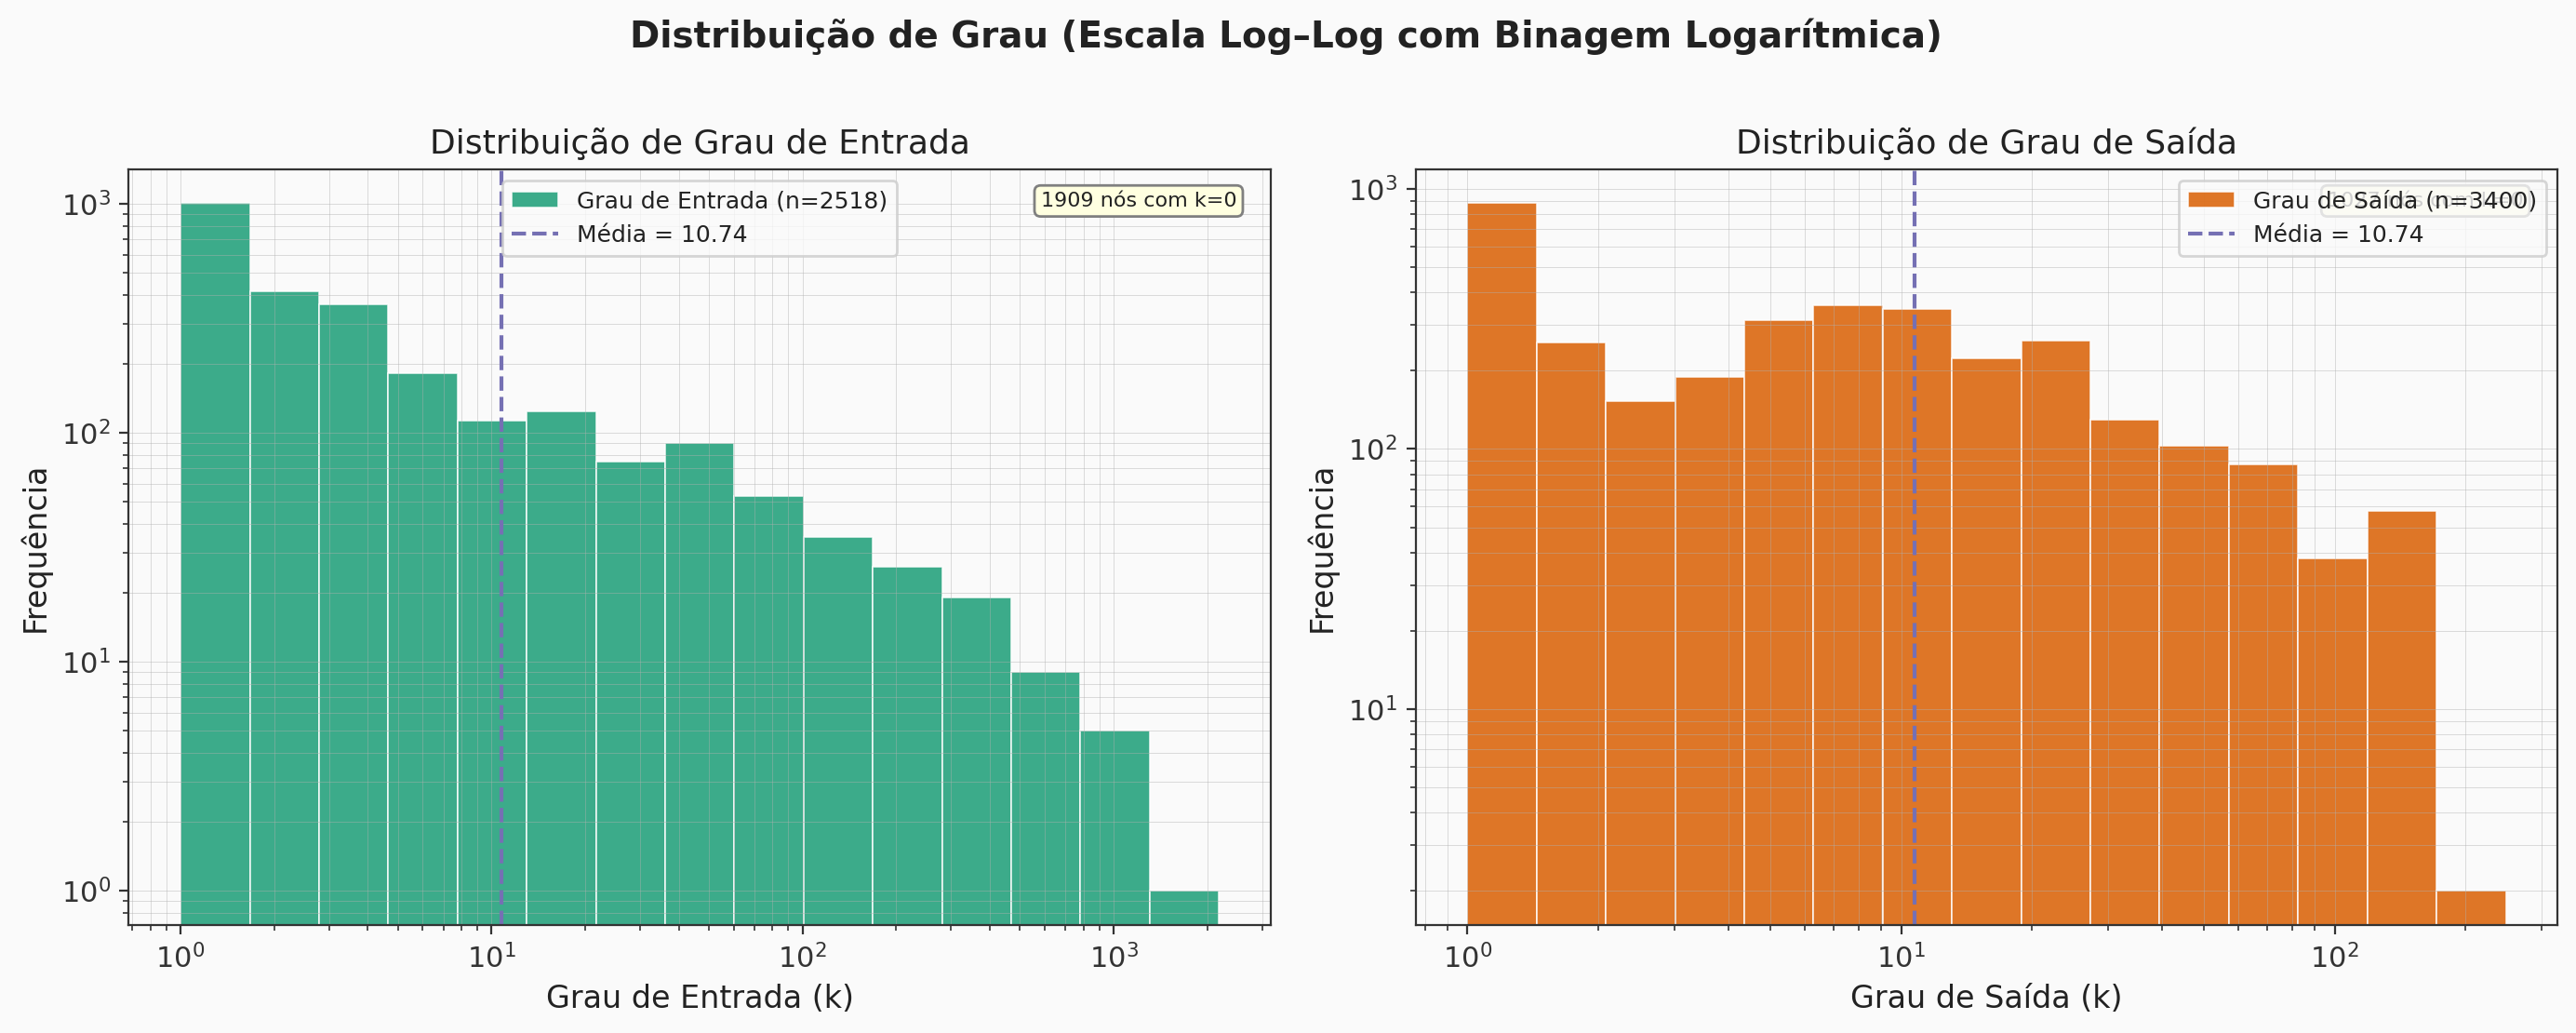
\includegraphics[width=\linewidth]{degree-distribution.png}
    \caption{Distribuição de grau (escala log--log).}
  \end{subfigure}\hfill
  \begin{subfigure}{0.48\textwidth}
    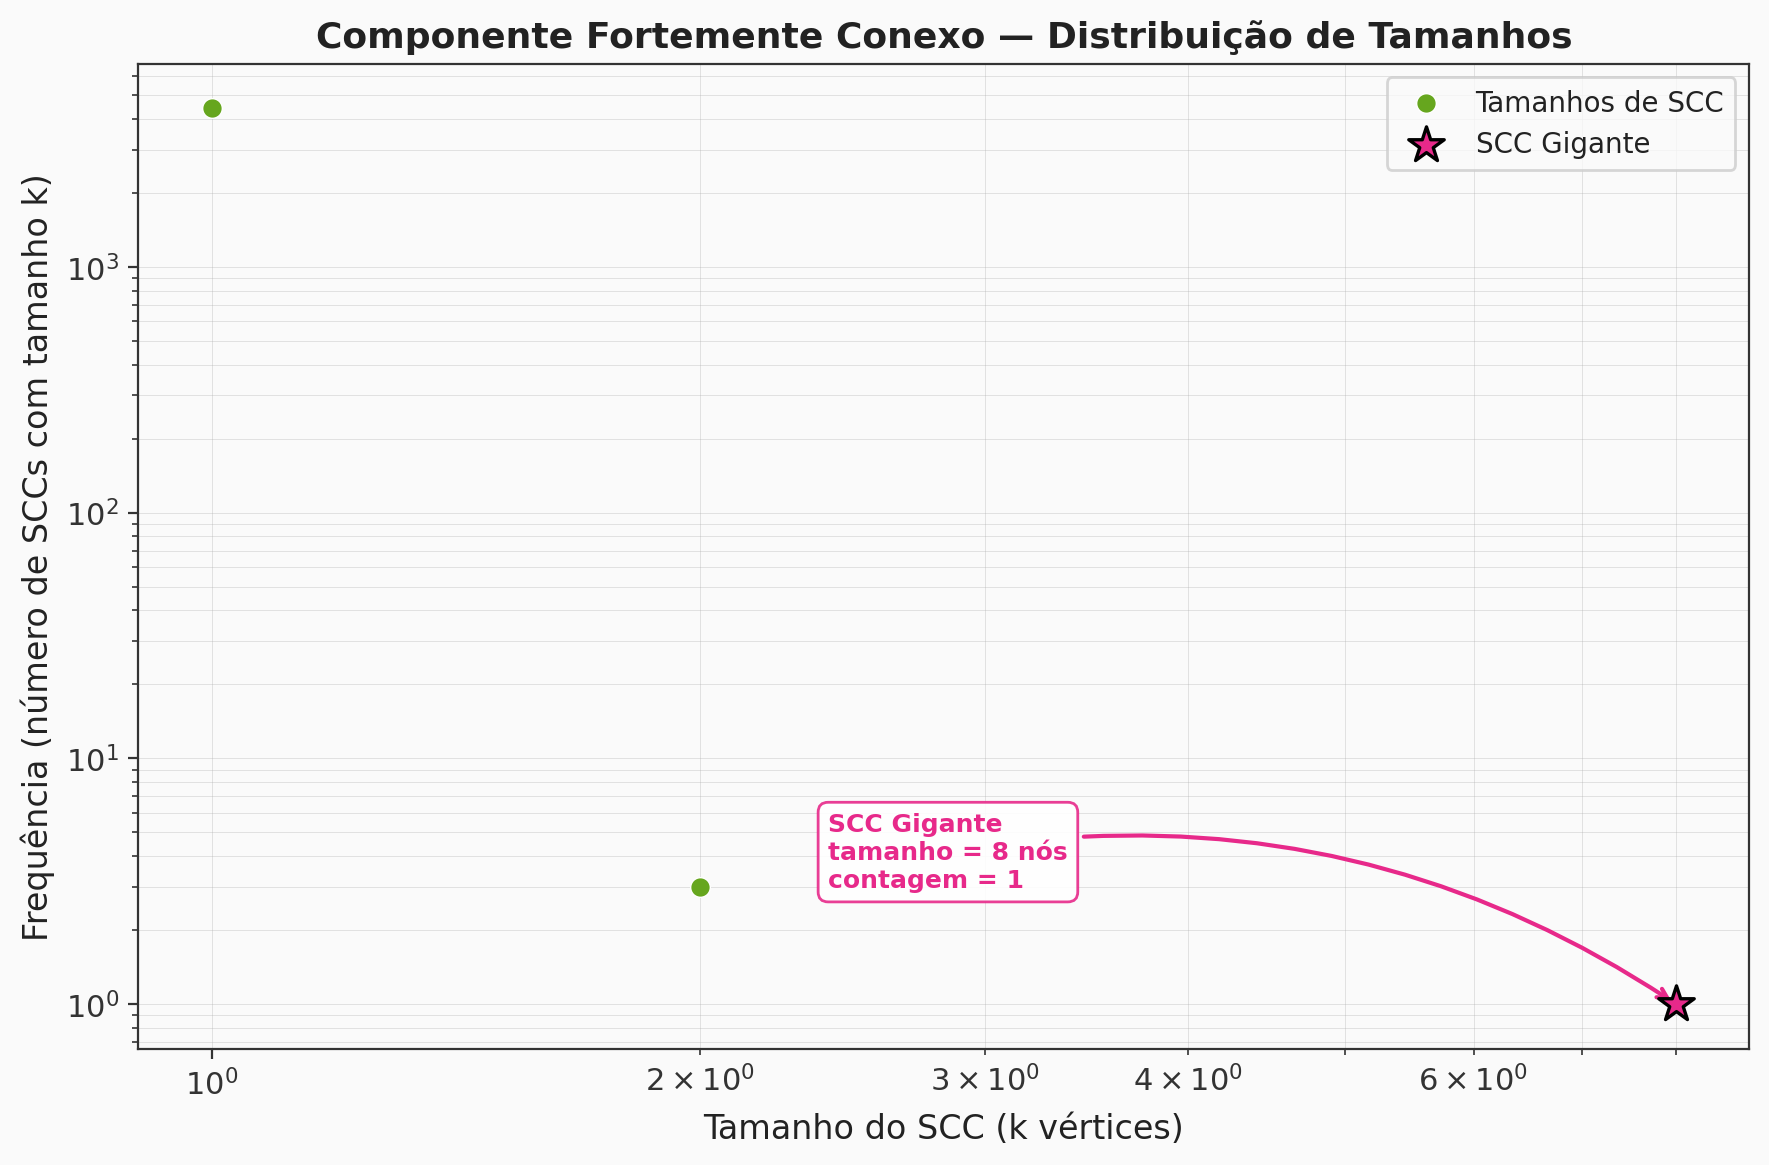
\includegraphics[width=\linewidth]{scc-distribution.png}
    \caption{Tamanho dos componentes fortemente conexos.}
  \end{subfigure}
  \caption{Caracterização estrutural do grafo de dependências. À esquerda, a
  assinatura livre de escala; à direita, a confirmação de que o grafo é quase
  acíclico (quase todos os SCCs têm tamanho 1).}
  \label{fig:carac}
\end{figure}

% ======================================================================
\section{Algoritmos e métodos}\label{sec:metodos}
% ======================================================================

O \emph{pipeline} tem quatro fases que se encadeiam: cada uma lê a saída da anterior.
Um ponto comum a todas as métricas é a normalização \emph{log-minmax}: antes de
qualquer combinação linear, aplica-se $\hat{x} = \big(\log(1+x) - \min\big)\,/\,
(\max-\min)$. Isso põe todas as componentes na mesma escala $[0,1]$ e, de novo,
domestica as caudas pesadas.

\subsection{Fase 1 --- score de risco $R(v)$}\label{sec:fase1}

O score de risco combina três sinais, cada um capturando uma faceta diferente de
``ser um alvo perigoso'':
\[
  R(v) = 0{,}35\,\hat{d}_{\text{in}}(v) \;+\; 0{,}25\,\hat{u}(v) \;+\; 0{,}40\,\hat{r}(v).
\]
Aqui $\hat{d}_{\text{in}}(v)$ é o grau de entrada normalizado (quantos pacotes
dependem \emph{diretamente} de $v$); $\hat{u}(v)$ é o uso normalizado (downloads); e
$\hat{r}(v)$ é o \emph{alcance transitivo}, isto é, quantos pacotes dependem de $v$
direta \emph{ou indiretamente} --- o ``raio de impacto'' de uma falha em $v$. Atribuiu-se o
maior peso (0,40) justamente ao alcance transitivo, porque é ele que traduz o
caráter sistêmico do risco: um pacote pode ter poucos dependentes diretos e, ainda
assim, sustentar meia floresta abaixo dele.

A parte algoritmicamente interessante é calcular o alcance transitivo de
\emph{todos} os nós de forma eficiente. Em vez de uma BFS reversa por nó (cara), usa-se
programação dinâmica sobre o grafo em ordem topológica, representando o conjunto de
ancestrais de cada nó como um \emph{bitarray} de $|V|$ bits. A união de dois conjuntos
vira um simples OU bit a bit, que o processador executa 64 bits por vez. Como o grafo
tem ciclos (poucos, mas existem), primeiro ele é condensado: cada SCC vira um
super-nó, roda-se a DP no DAG condensado --- garantidamente acíclico --- e depois
mapeia-se o resultado de volta para os nós originais. O Algoritmo~\ref{alg:reach}
resume o procedimento.

\begin{algorithm}[t]
\caption{Alcance transitivo via programação dinâmica em \emph{bitarrays}}
\label{alg:reach}
\begin{algorithmic}[1]
\Require grafo dirigido $G=(V,E)$, com $u\to v$ significando ``$u$ depende de $v$''
\Ensure $\text{reach}(v)$ = número de nós que dependem transitivamente de $v$
\If{$G$ possui ciclos}
  \State $G' \gets \textsc{Condensação}(G)$ \Comment{cada SCC vira um super-nó; $G'$ é um DAG}
\Else
  \State $G' \gets G$
\EndIf
\For{cada super-nó $w \in G'$}
  \State $\text{bits}[w] \gets$ bitarray de $|V|$ zeros, com 1 nas posições dos membros de $w$
\EndFor
\For{cada $v$ em ordem topológica de $G'$}
  \For{cada predecessor $u$ de $v$ em $G'$} \Comment{$u$ depende de $v$}
    \State $\text{bits}[v] \gets \text{bits}[v] \;\textbf{OU}\; \text{bits}[u]$
  \EndFor
\EndFor
\For{cada nó original $x \in V$}
  \State $\text{reach}(x) \gets \text{bits}[\,\text{super-nó de } x\,]\text{.contagem} - 1$
  \Comment{$-1$ remove o próprio $x$}
\EndFor
\State \Return $\text{reach}$
\end{algorithmic}
\end{algorithm}

\subsection{Fase 2 --- Criticidade $C(v)$ e score combinado $S(v)$}

A Fase 1 olha para o risco ``intrínseco'' de um pacote; a Fase 2 olha para a sua
\emph{posição estrutural} na rede. O índice de criticidade combina duas medidas
clássicas de centralidade:
\[
  C(v) = 0{,}40\,\hat{C}_D^{\text{in}}(v) \;+\; 0{,}60\,\widehat{PR}(v),
\]
em que $\hat{C}_D^{\text{in}}$ é a centralidade de grau de entrada e $\widehat{PR}$
é o PageRank (Brin \& Page, 1998). O PageRank é especialmente adequado aqui: como
ele propaga importância \emph{contra} o sentido das arestas, um pacote ganha
prestígio por ser dependência de pacotes que também são importantes --- exatamente a
noção de ``pacote fundacional'' que se procura.

Vale uma observação honesta sobre essa fórmula, porque ela não nasceu pronta ---
chegou-se a ela depois de tentar (e descartar) duas alternativas. A formulação inicial
do projeto tinha um terceiro termo, a \emph{betweenness} (centralidade de
intermediação), pensada para capturar ``gargalos'' --- pontes obrigatórias entre
regiões do grafo ---, com pesos $0{,}25 / 0{,}35 / 0{,}40$ para grau, betweenness e
PageRank. Ao medir, a ideia desmoronou. Num grafo quase acíclico quase não
existem pontes obrigatórias (ou há um caminho alternativo, ou não há caminho nenhum),
e o resultado foi que cerca de 97\% dos nós ficaram com betweenness exatamente zero.
Pior: a normalização min--max sobre um vetor quase todo nulo esticava o único nó
não-trivial para $1{,}0$, e isso bastava para alçar o \texttt{google-auth} --- que,
ironicamente, não tem nenhuma CVE registrada --- ao segundo lugar de criticidade. Era
um artefato numérico se disfarçando de achado.

A primeira correção foi simples: removeu-se a betweenness e redistribuiu-se o seu peso
entre os dois termos restantes, chegando à fórmula acima ($0{,}40 / 0{,}60$, com leve
favorecimento do PageRank, que é a medida de influência global teoricamente correta
para grafos dirigidos). Mas, antes de abandonar de vez a ideia de um termo estrutural,
optou-se por testar uma alternativa: existiria uma centralidade \emph{adequada} a um grafo
dirigido e quase acíclico? O candidato natural era a \textbf{centralidade de Katz}
(Katz, 1953), bem definida justamente onde a centralidade de autovetor degenera ---
em DAGs. Implementou-se um modo experimental que troca a betweenness por Katz (resolvida
por fatoração direta, sem risco de não-convergência), mantendo os pesos originais.

Não vingou, por dois motivos. Primeiro, não melhorou nada. Como a validação padrão da
Fase 4 mede só $R(v)$, foi preciso comparar as variantes à parte, validando a
criticidade \emph{pura} $C(v)$ diretamente contra o \emph{ground truth} do OSV; o Katz
ficou igual ou \emph{ligeiramente pior} que a versão sem termo estrutural
(Tabela~\ref{tab:variantes}). Segundo, e mais interessante: num DAG, a centralidade de
Katz se reduz a uma contagem atenuada de ancestrais --- ou seja, ela re-expressa boa
parte do \emph{alcance transitivo} que o score $R(v)$ já carrega. Seria contar
a mesma coisa duas vezes. A lição é que um caminho que não leva a lugar nenhum, quando
documentado, também é resultado: a versão atual fica com
$C(v) = 0{,}40\,\hat{C}_D^{\text{in}} + 0{,}60\,\widehat{PR}$, e os modos
\texttt{betweenness} e \texttt{katz} permanecem disponíveis apenas por trás de uma
chave de configuração, para reprodutibilidade.

\begin{table}[h]
\centering\small
\caption{Lift@$k$ (vulnerabilidade \emph{high}) da criticidade pura $C(v)$ sob as três
variantes do termo estrutural. A aparente vantagem da betweenness em $k=25$ e $50$ é de
um acerto a mais --- dentro do ruído amostral --- e não compensa nem o artefato do
\texttt{google-auth} nem o custo $O(V\cdot E)$. O Katz não supera a versão sem termo.}
\label{tab:variantes}
\begin{tabular}{crrr}
\toprule
$k$ & betweenness (falha)  & sem termo (atual) & Katz (experimental) \\
\midrule
10  & 10,6 & 10,6 & 10,6 \\
25  &  8,5 &  7,7 &  6,8 \\
50  &  7,7 &  6,8 &  6,4 \\
100 &  6,6 &  6,4 &  6,4 \\
\bottomrule
\end{tabular}
\end{table}

O score final que ordena os pacotes mistura risco e criticidade em partes iguais:
\[
  S(v) = 0{,}5\,R(v) + 0{,}5\,C(v).
\]

\subsection{Fase 3 --- Simulação de cascata (Modelo de Cascata Independente)}

Os scores anteriores são estáticos. Para responder ``\emph{o que aconteceria de
fato se este pacote fosse comprometido?}'' recorre-se a uma simulação estocástica:
o \textbf{Modelo de Cascata Independente} (ICM), emprestado da teoria de maximização
de influência em redes sociais (Kempe, Kleinberg \& Tardos, 2003).

A simulação roda sobre o grafo \emph{reverso}: se $u$ depende de $v$, uma
vulnerabilidade em $v$ ``infecta'' $u$ (que executa o código de $v$), então a
contaminação flui de $v$ para $u$. Cada aresta tem uma probabilidade de propagação
\[
  p(v \to u) = 0{,}01 + 0{,}99 \cdot R(v)\cdot \hat{u}(u),
\]
ou seja: um piso de 1\% (até dependências raras podem propagar um zero-day crítico),
escalado pelo risco da fonte e pelo uso do alvo. Partindo de um pacote-semente,
sorteia-se a propagação aresta a aresta em ondas, até nenhum novo nó ser infectado.
Como o processo é aleatório, repete-se $N=1000$ vezes (Monte Carlo) e toma-se a
média do tamanho final do conjunto infectado --- o \emph{raio de impacto esperado}
$\mathbb{E}[B(v)]$ --- junto com um intervalo de confiança de 95\%. O
Algoritmo~\ref{alg:icm} descreve uma rodada e a agregação.

\begin{algorithm}[t]
\caption{Simulação de cascata (ICM) com estimativa de Monte Carlo}
\label{alg:icm}
\begin{algorithmic}[1]
\Require grafo reverso $G^{T}$ com probabilidades $p(v\to u)$ pré-computadas; semente $s$; $N$ repetições
\Ensure raio de impacto esperado $\mathbb{E}[B(s)]$
\For{$i \gets 1$ \textbf{até} $N$}
  \State $\text{infectados} \gets \{s\}$;\quad $\text{fronteira} \gets \{s\}$
  \While{$\text{fronteira} \neq \varnothing$}
    \State $\text{nova} \gets \varnothing$
    \For{cada nó $w \in \text{fronteira}$}
      \For{cada vizinho $u$ de $w$ em $G^{T}$ com $u \notin \text{infectados}$}
        \If{$\textsc{Aleatório}(0,1) < p(w \to u)$}
          \State adicione $u$ a $\text{infectados}$ e a $\text{nova}$
        \EndIf
      \EndFor
    \EndFor
    \State $\text{fronteira} \gets \text{nova}$
  \EndWhile
  \State $B_i \gets |\text{infectados}|$
\EndFor
\State \Return $\frac{1}{N}\sum_{i=1}^{N} B_i$
\end{algorithmic}
\end{algorithm}

\subsection{Fase 4 --- Validação contra dados reais (OSV.dev)}

De nada adianta um ranking bonito se ele não bate com a realidade. A Fase 4 testa se
os pacotes que o modelo aponta como mais arriscados são, de fato, os que mais
acumulam vulnerabilidades reais. A metodologia separa dois grupos:
\textbf{Grupo A}, os 1.000 pacotes de maior $R(v)$; e \textbf{Grupo B}, 1.000 pacotes
sorteados aleatoriamente do restante, que funciona como grupo de controle para
estimar a taxa-base de vulnerabilidade do ecossistema. As métricas usadas foram:

\begin{itemize}\setlength\itemsep{1pt}
  \item \textbf{Correlação} (Spearman e Kendall, calculadas no Grupo B para evitar
        viés de restrição de amplitude), medindo se mais risco anda junto com mais
        vulnerabilidades.
  \item \textbf{Correlação parcial} controlando popularidade, para isolar se a
        \emph{topologia} prediz vulnerabilidades independentemente do número de
        downloads.
  \item \textbf{Precision@$k$ e Lift@$k$} para $k\in\{10,25,50,100\}$: das $k$
        cabeças do ranking, que fração é de fato vulnerável, e quantas vezes isso
        supera a taxa-base (o \emph{lift}).
  \item \textbf{Teste U de Mann--Whitney}, não-paramétrico, comparando a distribuição
        de vulnerabilidades dos dois grupos.
  \item \textbf{Robustez}: análise de sensibilidade ao limiar de CVSS e intervalos
        de confiança por \emph{bootstrap} (10.000 reamostragens).
\end{itemize}

% ======================================================================
\section{Resultados}\label{sec:resultados}
% ======================================================================

O \emph{pipeline} completo roda em poucos minutos. Os resultados são apresentados na
ordem das fases.

\paragraph{Fase 1 --- quem são os pacotes mais arriscados.}
O topo do ranking de $R(v)$ é, tranquilizadoramente, uma lista de quem qualquer
pessoa que programa em Python reconhece de imediato: infraestrutura de tipagem, HTTP,
TLS e \emph{parsing}. A Tabela~\ref{tab:risco} mostra os dez primeiros. Que o modelo
recupere espontaneamente esses ``pilares'' do ecossistema é um primeiro sinal de
sanidade --- são justamente os pontos únicos de falha que a proposta queria achar.

\begin{table}[h]
\centering\small
\caption{Top-10 por score de risco $R(v)$ (Fase 1).}
\label{tab:risco}
\begin{tabular}{clrrr}
\toprule
\# & Pacote & Grau entrada & Alcance ($r$) & $R(v)$ \\
\midrule
1 & \texttt{typing-extensions} & 2.181 & 2.188 & 0,984 \\
2 & \texttt{idna}              & 1.165 & 1.171 & 0,925 \\
3 & \texttt{certifi}           & 1.100 & 1.102 & 0,919 \\
4 & \texttt{urllib3}           & 1.001 & 1.003 & 0,910 \\
5 & \texttt{requests}          &   906 &   908 & 0,900 \\
6 & \texttt{charset-normalizer}&   920 &   922 & 0,899 \\
7 & \texttt{packaging}         &   777 &   782 & 0,888 \\
8 & \texttt{six}               &   693 &   696 & 0,865 \\
9 & \texttt{python-dateutil}   &   580 &   583 & 0,849 \\
10& \texttt{pyyaml}            &   509 &   509 & 0,835 \\
\bottomrule
\end{tabular}
\end{table}

\paragraph{Fase 2 --- criticidade e score combinado.}
Ao incorporar PageRank e grau, a ordenação por $S(v)$ permanece muito parecida, com
o \texttt{typing-extensions} isolado na liderança (score combinado $0{,}99$,
contra $\approx 0{,}60$ do segundo colocado). Esse abismo entre o primeiro e os
demais já antecipa o achado da fase seguinte: há um nó claramente em uma categoria
própria de importância estrutural.

\paragraph{Fase 3 --- o raio de impacto.}
Este é o resultado considerado mais relevante do trabalho
(Tabela~\ref{tab:cascata}). Comprometer um único pacote, o \texttt{typing-extensions},
contaminaria em média \textbf{1.507 pacotes --- cerca de 34\% de todo o grafo} --- em
pouco mais de três saltos. Os cinco pacotes seguintes sozinhos já colocam entre 12\%
e 20\% do ecossistema em risco cada um. É a confirmação quantitativa, no recorte do
PyPI, do fenômeno que Zimmermann et al. (2019) batizaram de ``mundo pequeno com
altos riscos''.

\begin{table}[h]
\centering\small
\caption{Raio de impacto esperado por semente (Fase 3, ICM com $N=1000$).}
\label{tab:cascata}
\begin{tabular}{lrrr}
\toprule
Semente & $\mathbb{E}[B]$ & \% do grafo & Profundidade média \\
\midrule
\texttt{typing-extensions} & 1.507 & $\sim$34\% & 3,09 \\
\texttt{idna}              &   881 & $\sim$20\% & 3,11 \\
\texttt{certifi}           &   821 & $\sim$18\% & 3,15 \\
\texttt{urllib3}           &   715 & $\sim$16\% & 3,18 \\
\texttt{charset-normalizer}&   668 & $\sim$15\% & 3,27 \\
\texttt{requests}          &   521 & $\sim$12\% & 3,28 \\
\bottomrule
\end{tabular}
\end{table}

\paragraph{Fase 4 --- o ranking bate com a realidade?}
Consultou-se o OSV.dev para os 2.000 pacotes dos dois grupos; \textbf{253 (12,7\%)}
tinham ao menos um \emph{advisory} e 197 tinham vulnerabilidade de alta severidade
(CVSS $\geq 7$). A taxa-base de vulnerabilidade \emph{high} no grupo de controle é de
apenas $4{,}7\%$. Contra esse pano de fundo, os números de enriquecimento são
expressivos (Tabela~\ref{tab:validacao}): entre os 10 pacotes mais arriscados, metade
já teve uma vulnerabilidade grave --- um \emph{lift} de \textbf{10,6$\times$} sobre o
acaso --- e o efeito se mantém forte até $k=100$. O teste de Mann--Whitney separa os
dois grupos com significância esmagadora ($p \approx 10^{-20}$). Por outro lado, e isso
merece honestidade, as correlações contínuas (Spearman, Kendall e a correlação
parcial) \emph{falharam} --- esse ponto, mais interessante do que
parece, é retomado na análise.

\begin{table}[h]
\centering\small
\caption{Resultados da validação contra o OSV.dev (Fase 4). Critério de aprovação
entre parênteses.}
\label{tab:validacao}
\begin{tabular}{lrl}
\toprule
Teste & Valor & Veredito \\
\midrule
Spearman $\rho$ (Grupo B) & $-0{,}022$ ($p=0{,}49$) & reprovado ($\rho>0{,}3$) \\
Kendall $\tau$ (Grupo B)  & $-0{,}017$ ($p=0{,}50$) & reprovado \\
Correlação parcial (controla uso) & $-0{,}085$ ($p=0{,}007$) & reprovado ($\rho>0{,}15$) \\
Mann--Whitney $U$ (A vs.\ B) & $p\approx 9{,}4\times10^{-20}$ & \textbf{aprovado} \\
Precision@10 (\emph{high}) & 50\% & --- \\
Lift@10 / @25 / @50 / @100 & 10,6$\times$ / 7,7$\times$ / 6,8$\times$ / 5,7$\times$ & \textbf{aprovado} (@25$>$3) \\
Sensibilidade ao limiar CVSS & 4/4 limiares com Lift@25$>$3 & robusto \\
\bottomrule
\end{tabular}
\end{table}

% ======================================================================
\section{Análise, interpretação e descobertas}\label{sec:analise}
% ======================================================================

À primeira vista, a Fase 4 parece contraditória: como o modelo pode ``passar
arrasador'' em \emph{lift} e Mann--Whitney e, ao mesmo tempo, ``falhar'' na
correlação de Spearman? A resposta --- e essa foi a descoberta conceitual mais
valiosa do projeto --- é que os dois grupos de testes medem coisas diferentes, e o
contraste entre eles diz muito sobre a natureza do problema.

\paragraph{O modelo é um classificador de cauda, não um termômetro contínuo.}
A variável-alvo (número de vulnerabilidades por pacote) é \emph{fortemente inflada em
zeros}: com taxa-base de 6\%, cerca de 94\% dos pacotes do grupo de controle têm
exatamente zero \emph{advisories}, e a mediana é 0 nos dois grupos. O coeficiente de
Spearman calculado sobre um vetor que é 94\% empate em zero converge para perto de
zero por construção --- ele está medindo ruído de ordenação dentro de uma massa de
zeros, não ausência de sinal. O sinal \emph{existe e é forte}, mas vive na cauda
extrema da distribuição, que é precisamente o que Precision@$k$, Lift@$k$ e
Mann--Whitney capturam. Em termos práticos: o modelo não serve para dizer ``o pacote
X é 1,3 vez mais arriscado que o Y'', mas é excelente para responder ``por onde a
equipe de segurança deve começar a auditar'' --- e é exatamente para isso que ele foi
pensado.

\paragraph{E, afinal, o que significa ``mais vulnerável''?}
Há ainda uma dificuldade conceitual, anterior aos dados, em querer um termômetro
contínuo. Dizer que ``o pacote X é mais vulnerável que o Y'' pressupõe que
vulnerabilidade seja uma grandeza bem-ordenada, e ela não é: depende de uma porção de
fatores que um modelo baseado em estrutura e popularidade sequer enxerga. Uma
vulnerabilidade exposta por um pacote pode morar num trecho de código que os seus
dependentes nunca chegam a chamar; ou pode ser \emph{neutralizada} na implementação de
quem o usa --- por exemplo, um dependente que valida a entrada antes de repassá-la, que
isola a chamada, ou que já fixou a versão corrigida ---, de modo que, na prática, não
há problema algum a jusante. Pesam também a severidade real da falha, a existência de
um \emph{exploit} público, se o caminho vulnerável é de fato alcançável em produção e a
velocidade com que a correção se propaga pela cadeia. Nada disso se reduz ao número de
downloads ou à posição no grafo. Ou seja: insistir num score contínuo e absoluto de
``vulnerabilidade'' seria prometer uma precisão que o problema simplesmente não
comporta. É mais um motivo para tratar o modelo pelo que ele faz bem --- ordenar
prioridades de auditoria --- em vez de exigir dele uma probabilidade que dependeria de
informação que nenhum grafo de dependências, sozinho, contém.

\paragraph{Um resultado negativo honesto: topologia não é independente de
popularidade.}
A correlação parcial controlando o número de downloads deu $-0{,}085$ ---
estatisticamente significativa, porém negativa. Pela hipótese ``forte'' do projeto,
esperava-se que a estrutura do grafo (grau + alcance) predissesse vulnerabilidades
mesmo depois de descontado o efeito de popularidade. Os dados não sustentam isso.
A leitura mais provável é a \textbf{Lei de Linus} (o famoso ``\emph{given enough
eyeballs, all bugs are shallow}''): pacotes muito populares recebem mais escrutínio e,
por isso, têm mais CVEs \emph{descobertas} --- não necessariamente são mais
inseguros. O sinal preditivo, neste recorte, mora na popularidade, e a topologia
residual não acrescenta poder.

\paragraph{O \emph{ground truth} é esparso e atrasado.}
Há ainda uma ressalva importante para interpretar os 12,7\% de pacotes com
\emph{advisory}: ausência de CVE não é prova de segurança. Alfadel et al. (2023)
mostram que vulnerabilidades em pacotes Python levam, em média, mais de três anos para
serem descobertas. Ou seja, boa parte dos ``zeros'' do \emph{ground truth} são
provavelmente vulnerabilidades ainda não descobertas. Isso põe um teto desconhecido
em qualquer correlação contínua e reforça por que o enriquecimento (priorização) é a
métrica certa para este tipo de dado.

\paragraph{Onde o trabalho conversa com a literatura.}
Os números de \emph{lift} de 6 a 11 vezes estão na mesma direção dos resultados de
priorização por métricas de Shin et al.\ (2011) e Zimmermann \& Nagappan (2008),
ainda que os valores absolutos não sejam diretamente comparáveis (granularidades e
taxas-base distintas). O raio de impacto de $\sim$34\% num único pacote é o mesmo
fenômeno estrutural descrito por Zimmermann et al.\ (2019) para o npm, em escala
proporcional ao subgrafo. E a propagação transitiva em poucos saltos ecoa
Decan et al.\ (2018).

% ======================================================================
\section{Conclusão}
% ======================================================================

Este trabalho apresentou um \emph{pipeline} que parte de dados públicos do
PyPI, construído de ponta a ponta, monta um grafo de 4.427 pacotes, atribui a cada um
deles um score de risco e de criticidade, simula a propagação de uma vulnerabilidade e
valida o ranking contra CVEs reais. O modelo cumpre bem o objetivo para o qual foi desenhado --- priorizar
pacotes para auditoria ---, identificando os pontos únicos de falha do ecossistema com
uma taxa de acerto de 6 a 11 vezes acima do acaso para vulnerabilidades graves. A
simulação de cascata quantificou de forma concreta o risco sistêmico: o
comprometimento do \texttt{typing-extensions} alcançaria, em expectativa, um terço de
todo o grafo.

Tão importante quanto os acertos foram as limitações que o experimento expôs: o modelo é um classificador de cabeça de cauda, e não um estimador contínuo;
e, neste recorte de dados, a estrutura do grafo não se mostrou um preditor de
vulnerabilidades independente da popularidade. Longe de enfraquecer o trabalho,
esses resultados negativos --- somados ao reconhecimento de que a betweenness é
inadequada num grafo quase acíclico --- foram o que mais ensinou sobre o problema.
Como direções futuras, valeria ampliar o grafo para incluir a verdadeira cauda do
PyPI (dando variância de desfecho às correlações), calibrar os pesos e as
probabilidades contra dados históricos e adotar modelos estatísticos próprios para
dados inflados em zero.

% ======================================================================
\begin{thebibliography}{9}
\small
\bibitem{brinpage} Brin, S.; Page, L. (1998). \emph{The Anatomy of a Large-Scale
Hypertextual Web Search Engine.} Computer Networks, 30(1--7), 107--117.
\bibitem{brandes} Brandes, U. (2001). \emph{A Faster Algorithm for Betweenness
Centrality.} Journal of Mathematical Sociology, 25(2), 163--177.
\bibitem{katz} Katz, L. (1953). \emph{A new status index derived from sociometric
analysis.} Psychometrika, 18(1), 39--43.
\bibitem{kempe} Kempe, D.; Kleinberg, J.; Tardos, É. (2003). \emph{Maximizing the
Spread of Influence through a Social Network.} KDD 2003.
\bibitem{smallworld} Zimmermann, M.; Staicu, C.-A.; Tenny, C.; Pradel, M. (2019).
\emph{Small World with High Risks: A Study of Security Threats in the npm Ecosystem.}
USENIX Security 2019.
\bibitem{decan} Decan, A.; Mens, T.; Constantinou, E. (2018). \emph{On the Impact of
Security Vulnerabilities in the npm Package Dependency Network.} MSR 2018.
\bibitem{alfadel} Alfadel, M.; Costa, D. E.; Shihab, E. (2023). \emph{Empirical
analysis of security vulnerabilities in Python packages.} Empirical Software
Engineering, 28, 59.
\bibitem{zimnagappan} Zimmermann, T.; Nagappan, N. (2008). \emph{Predicting Defects
using Network Analysis on Dependency Graphs.} ICSE 2008.
\bibitem{shin} Shin, Y.; Meneely, A.; Williams, L.; Osborne, J. (2011).
\emph{Evaluating Complexity, Code Churn, and Developer Activity Metrics as Indicators
of Software Vulnerabilities.} IEEE TSE, 37(6).
\bibitem{cvss} FIRST.Org (2019). \emph{Common Vulnerability Scoring System (CVSS) v3.1
Specification.}
\bibitem{osv} Google Open Source (2021--). \emph{OSV.dev --- Open Source
Vulnerabilities database.} \url{https://osv.dev}
\bibitem{depsdev} Google (2021--). \emph{deps.dev / BigQuery public datasets
(\texttt{deps\_dev\_v1}, \texttt{pypi.file\_downloads}).}
\end{thebibliography}

\end{document}
